\section{Modeling with ordinary differential equations}

\begin{example}[Exponential growth]
  Bacteria are living on a substrate with ample nutrients. Each
  bacteria splits into two after a certain time $\Delta t$. The time
  span for splitting is fixed and independent of the individuum. Then,
  given the amount $u_0$ of bacteria at time $t_0$, the amount at
  $t_1 = t_0+\Delta t$ is $u_1 = 2 u_0$. Generalizing, we obtain
  \begin{gather*}
    u_n = u(t_n) = 2^n u_0, \qquad t_n = t_0 + n\Delta t.
  \end{gather*}

  After a short time, the number of bacteria will be huge, such that
  counting is not a good idea anymore. Also, the cell division does
  not run on a very sharp clock, such that after some time, divisions
  will not only take place at the discrete times $t_0+n\Delta t$, but
  at any time between these as well. Therefore, we apply the continuum
  hypothesis, that is, $u$ is not a discrete quantity anymore, but a
  continuous one that can take any real value. In order to accommodate
  for the continuum in time, we make a change of variables:
  \begin{gather*}
    u(t) = 2^{\frac{t-t_0}{\Delta t}} u_0.
  \end{gather*}

  Here, we have already written down the solution of the problem,
  which is hard to generalize. The original description of the problem
  involved the change of $u$ from one point in time to the next. In
  the continuum description, this becomes the derivative, which we can
  now compute from our last formula:
  \begin{gather*}
    \tfrac{d}{dt} u(t) = \frac{\ln 2}{\Delta t} 2^{\frac{t-t_0}{\Delta t}} u_0
    = \frac{\ln 2}{\Delta t} u(t).
  \end{gather*}
  
  We see that the derivative of $u$ at a certain time depends on $u$
  itself at the same time and a constant factor, which we call the
  growth rate $\alpha$. Thus, we have arrived at our first
  differential equation
  \begin{gather}
    \label{eq:models:1}
    u'(t) = \alpha u(t).
  \end{gather}
  What we have seen as well is, that we had to start with some
  bacteria to get the process going. Indeed, any function of the form
  \begin{gather*}
    u(t) = c e^{\alpha t}
  \end{gather*}
  is a solution to equation~\eqref{eq:models:1}. It is the initial
  value $u_0$, which anchors the solution and makes it unique.
\end{example}

\begin{example}[Predator-prey systems]
  We add a second species to our bacteria example. Let's say, we
  replace the bacteria by sardines living in a nutrient rich sea, and
  we add tuna eating sardines. The amount of sardines eaten depends on
  the likelyhood that a sardine and a tuna are in the same place, and
  on the hunting efficiency of the tuna. Thus,
  equation~\eqref{eq:models:1} is augmented by a negative change in
  population depending on the product of sardines $u$ and tuna $v$:
  \begin{gather*}
    u' = \alpha u - \beta u v.
  \end{gather*}

  In addition, we need an equation for the amount of tuna. In this
  simple model, we will make two assumptions: first, tuna die of
  natural causes at a death rate of $\gamma$. Second, tuna procreate
  if there is enough food (sardines), and the procreation rate is
  proportional to the amount of food. Thus, we obtain
  \begin{gather*}
    v' = \delta u v - \gamma v.
  \end{gather*}

  Again, we will need initial populations at some point in time to
  compute ahead from there.
\end{example}

\begin{remark}
  The Lotka-Volterra-equations have periodic solutions. Even though
  none of these exist in closed form the sulotions can be simulated:
  \begin{center}
  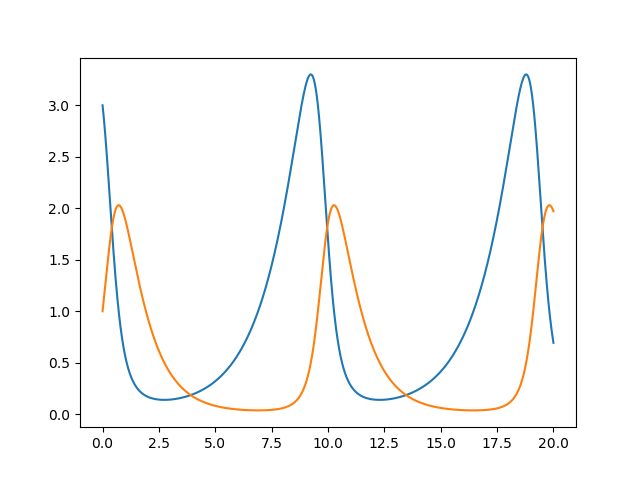
\includegraphics[width=.48\textwidth]{fig/lotkavolterra}
  \captionof{Plot of a solution to the Lotka-Volterra equation with
  parameters $\alpha = \frac 23$, $\beta  = \frac 43$, $\delta = \gamma = 1$
  and initial values $u(0) = 3$, $v(0) = 1$. Solved with a Runge-Kutta
  method of order five and step size $h = 10^{-5}$ \label{fig:lotkavolterra}}
  \end{center}
  Lotka and Volterra became interested in this system as they had
  found that the amount of predatory fish caught had increased
  during World War I. During the war years there was a strong
  decrease of fishing effort. In conclusion, they thought, there had
  to be more prey fish.
  
  A (far too rarely) applied consequence is that in order to diminish
  the amount of e.g. foxes one should hunt rabbits as foxes feed
  on rabbits.
\end{remark}

\begin{example}[Graviational two-body systems]
  According to Newton's law of universal gravitation, two bodies of
  masses $m_1$ and $m_2$ attract each other with a force
  \begin{gather*}
    \vec F_1 = G \frac{m_1m_2}{r^3} \vec r_1,
  \end{gather*}
  where $\vec F_1$ is the force vector acting on $m_1$ and $\vec r_1$
  is the vector pointing from $m_1$ to $m_2$ and $r = \lvert\vec r_1\rvert = \lvert\vec r_2\rvert$.

  Newton's second law of motion on the other hand relates forces and
  acceleration:
  \begin{gather*}
    \vec F = m \vec x'',
  \end{gather*}
  where $\vec x$ is the position of a body in space.

  Combining these, we obtain equations for the positions of the two bodies:
  \begin{gather*}
    \vec x''_i = G \frac{m_{3-i}}{r^3} (\vec x_i - \vec x_{3-i}), \qquad i=1,2.
  \end{gather*}
  This is a system of 6 independent variables. Nevertheless, it can be
  reduced to three by using that the center of mass moves
  inertially. Then, the distance vector is the only variable to be
  computed for:
  \begin{gather*}
    \vec r'' = - G \frac{m}{r^3} \vec r.
  \end{gather*}
  Intuitively, that we need an initial position and an initial
  velocity for the two bodies. Later on, we will see that this can
  actually be justified mathematically.
\end{example}

\begin{example}[Celestial mechanics]
  Now we extend the two-body system to a many-body system. Again, we
  subtract the center of mass, such that we obtain $n$ sets of 3
  equations for an $n+1$-body system. Since forces simply add up, this
  system becomes
  \begin{gather}
    \label{eq:celestial}
    \vec x_i = -G \sum_{j\neq i} \frac{m_j}{r_{ij}^3} \vec r_{ij}.
  \end{gather}
  Here, $\vec r_{ij} = \vec r_j - \vec r_i$ and $r_{ij} = \lvert \vec r_{ij}\rvert$.
  Initial data for the solar system can be obtained from
  \begin{center}
    \texttt{https://ssd.jpl.nasa.gov/?horizons}
  \end{center}
\end{example}

%%% Local Variables: 
%%% mode: latex
%%% TeX-master: "notes"
%%% End: 
